% !TEX root=../main.tex
\documentclass[../main]{subfiles}
\begin{document}
\chapter{はじめに}
\section{表}
\begin{table}[htbp]
  \begin{center}
  \caption{1学期期末テスト}
  \label{tab:mapping}
  \begin{tabular}{l|r}
      科目 & 点数 \\ \hline
      国語 & 60 \\
      算数 & 30 \\
      理科 & 40 \\
      社会 & 80
  \end{tabular}
  \end{center}
\end{table}

\section{画像}
\begin{figure}[htbp]
  \begin{center}
  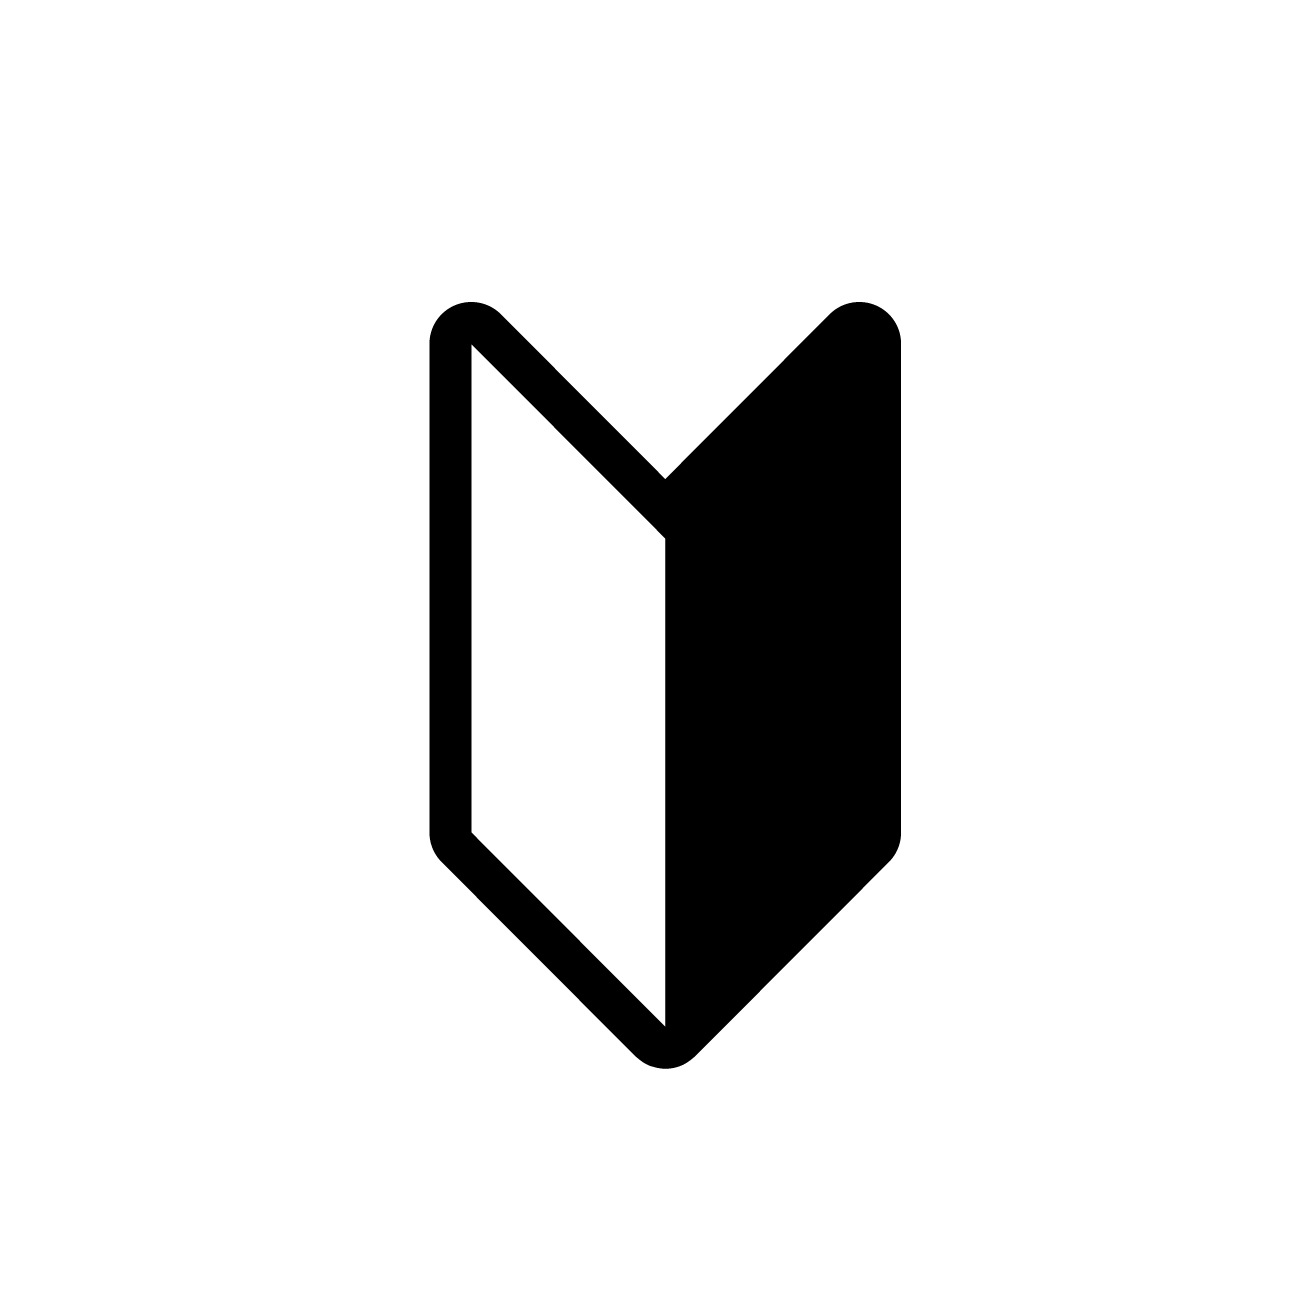
\includegraphics[width = 6cm,pagebox=cropbox]{./assets/images/163811.png}
  \caption{画像}
  \label{fig:sample-imaage}
  \end{center}
\end{figure}

\end{document}
